%The challenge of estimation is then to first overcome this intractability by means of a suitable approximation of the integral.
%Several methods may be employed, namely quadrature methods, Laplace approximation, and Markov chain Monte Carlo (MCMC) methods, but these all fail in the face of high dimensionality when the sample size $n$ is large.

As with the normal I-prior model, an estimate of the posterior regression function with optimised hyperparameters is sought.
The log likelihood function $L(\cdot)$ for $\theta$ using all $n$ observations $\{(y_1,x_1),\dots,(y_n,x_n)\}$ is obtained by integrating out the I-prior from the categorical likelihood, as follows:
\begin{align}
  L(\theta) 
  &= \log \int p(\by | \bw, \theta) \, p(\bw|\theta) \dint \bw \nonumber \\
  &= \log \int \prod_{i=1}^n \prod_{j=1}^m \Big( g_j^{-1}\big(\alpha_k + 
  \greyoverbrace{f_k(x_i)}{\hidewidth\sum_{i'=1}^n h_\eta(x_i,x_{i'})w_{i'k}\hidewidth}
  \,\big)_{k=1}^m \Big)^{[y_i=j]} \cdot \MN_{n,m}(\bw|\bzero,\bI_n, \bPsi) \dint \bw \label{eq:intractablelikelihood}
\end{align}
where we have denoted the probit relationship from \cref{eq:pij} using the function $g_j^{-1}:\bbR^m \to [0,1]$.
Unlike in the continuous response models, the integral does not present itself in closed form due to the conditional categorical PMF of the $y_i$'s, which they themselves involve integrals of multivariate normal densities.
For binary response models, $g^{-1}$ is simply the probit function, but for multinomial responses, this can be quite challenging to evaluate---more on this in \cref{sec:mnint}.

Furthermore, the posterior distribution of the regression function, which requires the density of $\bw|\by$, depends on the marginalisation provided by \cref{eq:intractablelikelihood}.
The challenge of estimation is then to first overcome this intractability by means of a suitable approximation of the integral.
We present three possible avenues to achieve this aim, namely the Laplace approximation, variational Bayes, and Markov chain Monte Carlo (MCMC) methods.

\subsection{Laplace approximation}

To compute the posterior density $p(\bw|\by) \propto p(\by|\bw)p(\bw) =: e^{Q(\bw)}$ with normalising constant equal to the marginal density of $\by$, $p(\by) = \int e^{Q(\bw)} \dint \bw$, we have established that this is intractable.
Laplace's method \citep[§4.1.1, pp. 777--778]{kass1995bayes} entails expanding a Taylor series for $Q$ about its posterior mode $\hat\bw = \argmax_\bw p(\by|\bw)p(\bw)$, which gives the relationship
\begin{align*}
  Q(\bw) 
  &= Q(\hat\bw) + 
  \cancelto{0}{(\bw - \hat\bw)^\top \nabla Q(\hat\bw)} 
  - \half (\bw - \hat\bw)^\top \bOmega (\bw - \hat\bw) + \cdots \\
  &\approx Q(\hat\bw) + 
  - \half (\bw - \hat\bw)^\top \bOmega (\bw - \hat\bw),
\end{align*}
because, assuming that $Q$ has a unique maxima, $\nabla Q$ evaluated at its mode is zero.
This is recognised as the logarithm of an unnormalised Gaussian density, implying $\bw|\by \sim \N_n(\hat\bw,\bOmega^{-1})$.
Here, $\bOmega = -\nabla^2 Q(\bw)|_{\bw=\hat\bw}$ is the negative Hessian of $Q$ evaluated at the posterior mode, and is typically obtained as a byproduct of the maximisation routine of $Q$ using gradient or quasi-gradient based methods.

The marginal distribution is then approximated by
\begin{align*}
  p(\by) 
  &\approx \int \exp
  \greyoverbrace{Q(\bw)}{\hidewidth Q(\hat\bw) - \half (\bw - \hat\bw)^\top \bOmega (\bw - \hat\bw)\hidewidth}
   \dint \bw \\
  &= (2\pi)^{n/2} \abs{\bOmega}^{-1/2} e^{Q(\hat\bw)} 
  \int (2\pi)^{-n/2} \abs{\bOmega}^{1/2} \exp \left(- \half (\bw - \hat\bw)^\top \bOmega (\bw - \hat\bw) \right) \dint\bw \\
  &= (2\pi)^{n/2} \abs{\bOmega}^{-1/2} p(\by|\hat\bw)p(\hat\bw).
%  &= \cancelto{1}{\int \phi(\bw|\hat\bw,\bOmega^{-1})}
\end{align*} 
The log marginal density of course depends on the parameters $\theta$, which becomes the objective function to maximise in a likelihood maximising approach.
Note that, should a fully Bayesian approach be undertaken, i.e. priors prescribed on the model parameters using $\theta \sim p(\theta)$, then this approach is viewed as a maximum a posteriori approach.

In any case, each evaluation of the objective function $L(\theta) = \log p(\by|\btheta)$ involves finding the posterior modes $\hat\bw$.
This is a slow and difficult undertaking, especially for large sample sizes $n$---even assuming computation of the class probabilities $g^{-1}$ is efficient---because the dimension of this integral is exactly the sample size.
Furthermore, obtaining standard errors for the parameters are cumbersome, and it is likely that a computationally burdensome bootstrapping approach is needed.
Lastly, as a comment, Laplace's method only approximates the true marginal likelihood well if the true function is small far away from the mode.

\subsection{Variational inference}

We turn to variational inference as a method of estimation. 
Variational methods are widely discussed in the machine learning literature, but there have been efforts to popularise it in statistics \citep{blei2017variational}.
In a fully Bayesian setting, one obtains an approximation to the intractable posterior distribution of interest, which is then used for inferential purposes in lieu of the actual posterior distribution.

In addition to the I-probit model, suppose that prior distributions are assigned on the hyperparameters of the model, $\theta \sim p(\theta)$.
By appending the latent variables $\{\by^*,\bw\}$ to the hyperparameters $\theta$, we seek an approximation
\[
  p(\by^*,\bw,\theta | \by) \approx \tilde q(\by^*,\bw,\theta),
\]
where $\tilde q$ satisfies $\tilde q = \argmin_q \KL(q\Vert p)$, subject to certain constraints.
The constraint considered by us in this thesis is that $q$ satisfies a \emph{mean-field} factorisation
\[
  q(\by^*,\bw,\theta) = q(\by^*)q(\bw)q(\theta).
\]
Under this scheme, the posterior for $\by^*$ is found to be a \emph{conically truncated multivariate normal} distribution, and for $\bw$, a multivariate normal distribution.
The posterior density $q(\theta)$ is often of a recognisable form, and usually one of the exponential family densities (normal, Wishart or gamma).
This is useful, because point estimates of the hyperparameters can be taken to be either the mean or mode of these well-known distributions.
In cases where $q(\theta)$ does not conform to an exponential family type density, then inference can still be done by sampling methods.

It can be shown that, for some variational density $q$, the marginal log-likelihood is an upper-bound for the quantity $\cL$
\[
  \log p(\by) \geq 
    \E_{ q} \log p(\by,\by^*,\bw,\theta)
    - \E_{ q} \log \tilde q(\by^*,\bw,\theta) =: \cL,
%  }{\cL},
\]
a quantity often referred to as the \emph{evidence lower bound} (ELBO).
It turns out that minimising $\KL(q\Vert p)$ is equivalent to maximising the ELBO, a quantity that is more practical to work with than the KL divergence.
That is, if $\tilde q$ approximates the true posterior well, then the ELBO is a suitable proxy for the maximised marginal log-likelihood.

The algorithm to obtain $\tilde q$ which maximises the ELBO is known as the \emph{coordinate ascent variational inference} (CAVI) algorithm.
The algorithm itself typically condenses to that of a simple, sequential updating scheme, akin to the expectation-maximisation (EM) algorithm for exponential families we saw in Chapter 4, which is very fast to implement compared to the other methods described in the previous subsections.
A full derivation of the variational algorithm used by us will be described in \cref{sec:iprobitvar}.
%\citep{mclachlan2007algorithm}

\subsection{Markov chain Monte Carlo methods}

As an alternative to the deterministic Bayesian approach of variational inference, it is possible to use Markov chain Monte Carlo sampling methods as an approach to stochastically approximate the intractable posterior distribution.

\citet{albert1993bayesian} showed that the latent variable approach to probit models can be analysed using exact Bayesian methods, due to the underlying normality structure.
Paired with corresponding conjugate prior choices, sampling from the posterior is very simple using a Gibbs sampling approach.
On the other hand, this data augmentation scheme enlarges the variable space to $n+q$ dimensions, where $q$ is the number of parameters to estimate, which is inefficient and computationally challenging especially when $n$ is large.
It is no longer possible to marginalise the normal latent variables from the model, as this is intractable, as discussed previously.

Hamiltonian Monte Carlo is another possibility, since it does not require conjugacy.
For binary models, this is a feasible approach because the class probabilities are a function of the normal CDF, which means that it is doable using off-the-shelf software such as \proglang{Stan}.
However, with multinomial responses, the arduous task of computing class probabilities, which involve integration of an at most $m$-dimensional normal density, must be addressed separately.

%In summary, the computational challenge here stems from two sources: 1) integrating out the random effects $\bw$; and 2) evaluating class probabilities.
%Point 1) is addressed using a Gibbs sampling data augmentation scheme (latent variable approach), but this is not feasible with large $n$.
%Point 2) remains regardless whether Gibbs sampling or HMC is used.

\subsection{Comparison of estimation methods}

In this subsection, we utilise a toy binary classification data set which has been simulated according to a spiral pattern, as in \cref{fig:exampleiprobit}.
The predictor variables are $X_1$ and $X_2$, each of which are scaled similarly.

\begin{figure}[hbt]
  \centering
  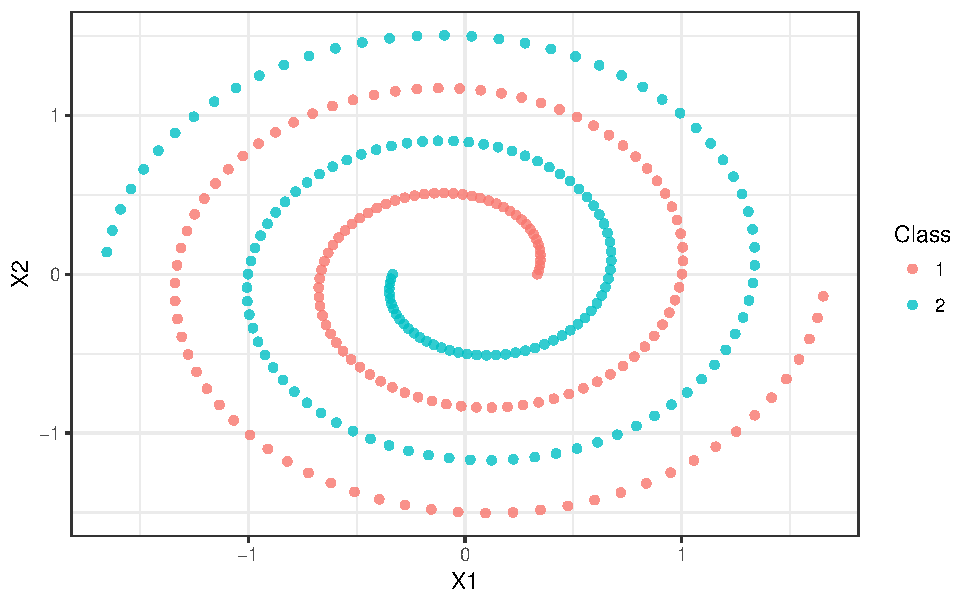
\includegraphics[width=0.8\textwidth]{figure/05-example_data}
  \caption{A plot of simulated spiral data set.}
  \label{fig:exampleiprobit}
\end{figure}

The I-probit model that is fitted is
\begin{gather*}
  y_i \sim \Bern(p_i) \\
  \Phi^{-1}(p_i) = \alpha + \sum_{k=1}^n h_\lambda(x_i,x_k)w_k  \\
  w_1,\dots,w_n \iid \N(0,1).
\end{gather*}
This binary model follows from the more general multinomial I-probit model by fixing all latent propensities in one of the classes to zero, and setting $\bPsi = \bI_m$.
This is possible because only differences in latent propensities are of interest, and not the actual values themselves, and thus only $m-1$ sets of posterior regression functions need to be estimated---see \cref{sec:mnint} for further details.

The three estimation methods described aim to overcome the intractable integral by means of either a deterministic approximation (Laplace and variational inference) or a stochastic approximation (Hamiltonian MC).
For the Bayesian methods, i.e. variational inference and Hamiltonian MC, vague priors were used on $\alpha$ and $\lambda$, namely $\N(0,100)$ and $\N_+(0,100)$ respectively.
Restriction of $\lambda$ to the positive orthant is required for identifiability.
The Laplace and variational methods were performed in the \pkg{iprobit} package, while \proglang{Stan} was used to code the Hamiltonian MC sampler.
The results are presented in \cref{tab:compreiprobit}.

\begin{table}[hbt]
\centering
\caption{Table comparing the estimated parameter values, (marginal) log-likelihood values, and also time taken for the three estimation methods.}
\label{tab:compreiprobit}
\begin{tabular}{@{}lrrr@{}}
\toprule
& Laplace approximation 
& Variational inference 
& Hamiltonian MC          \\ \midrule
Intercept ($\alpha$)      & -0.02 (0.03)           & 0.00 (0.06)    & 0.00 (0.58)  \\
Scale ($\lambda$)      & 0.85 (0.01)         & 5.67 (0.23)  & 29.3 (5.21)     \\[0.5em]
Log density    & -202.7              & -140.7       & -163.8                  \\
Error rate (\%) & 44.7               & 0.00        & 2.24                   \\
Brier score & 0.20               & 0.02        & 0.01                   \\[0.5em]
Iterations     & 20                  & 56          & 2000                    \\
Time taken (s) & >3600                & 5.32         & >3600                     \\ \bottomrule
\end{tabular}
\end{table}

The three methods pretty much concur on the estimation of the intercept, but not on the RKHS scale parameter.
As a result, the log-density value at the optima is also different in all three methods.
Notice the high posterior standard deviation for the scale parameter in the HMC method.
The posterior density for $\lambda$ was very positively skewed, and this contributed to the large posterior mean.

A plot of the log-likelihood surface for three methods in \cref{fig:exampleiprobitfit} reveals some insight.
The variational likelihood reveals two ridges, with the maxima occurring around the intersection of these two ridges.
The Laplace likelihood seems to indicate a similar shape---in both the Laplace and variational method, the posterior distribution of $\bw$ is approximated by a Gaussian distribution, with different means and variances.
However, parts of the Laplace likelihood are poorly approximated resulting in a loss of fidelity around the supposed maxima, which might have contributed to the set of values that were estimated.
Laplace's method is known to yield poor approximations to probit-type likelihoods, as studied by \citet{kuss2005assessing}.
On the other hand, the log-likelihood using the posterior distribution of the Hamiltonian MC sampler (treating parameters as fixed values) yields a completely different shape compared to the other two methods.

In terms of predictive abilities, both the variational and Hamiltonian MC methods, even though the posteriors are differently estimated, has good predictive performance as indicated by their error rates and Brier scores.
\cref{fig:exampleiprobitfit} shows that HMC is more confident of new data predictions compared to variational inference, as indicated by the intensity of the shaded regions (HMC is stronger than VI).
Laplace's method gave poor predictive performance.

Finally, on the computational side, variational inference was by far the fastest method to fit the model.
Sampling using Hamiltonian MC was very slow, because the parameter space is in effect $O(n + 2)$ (parameters are $\{w_1,\dots,w_n,\alpha,\lambda\}$), and unlike in the normal model, we are not able to easily marginalise out the I-prior.
As for Laplace, each Newton step involves obtaining posterior modes of the $w$'s, and this contributed to the slowness of this method.
The reality is that variational inference takes seconds to complete what either the Laplace or full MCMC methods would take hours to.
The predictive performance, while not as good as HMC, is certainly an acceptable compromise in favour of speed.

\begin{figure}[p]
  \centering
  \vspace{1em}
  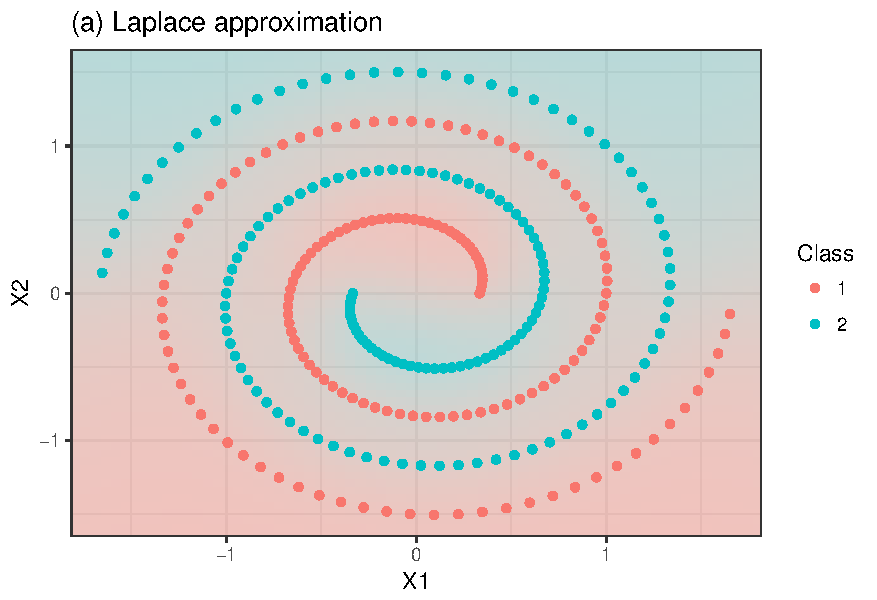
\includegraphics[width=0.49\textwidth]{figure/05-fit_lap}
  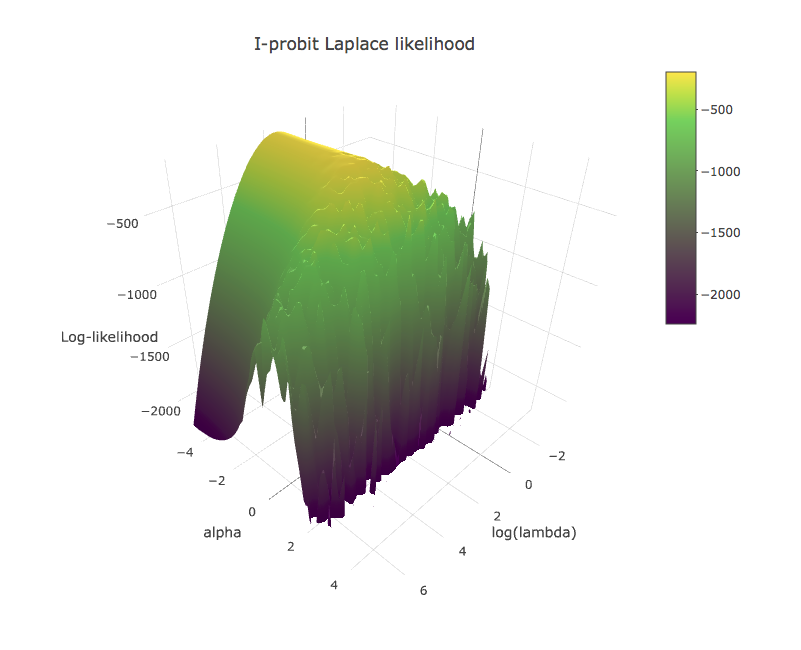
\includegraphics[width=0.49\textwidth]{figure/05-lik_lap}
  \vspace{1em}
  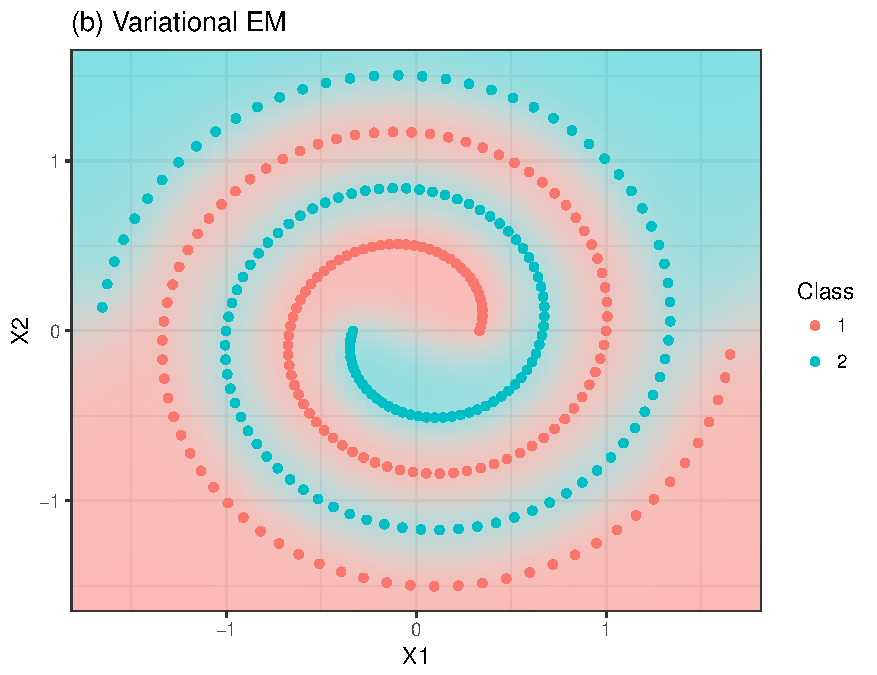
\includegraphics[width=0.49\textwidth]{figure/05-fit_vi}
  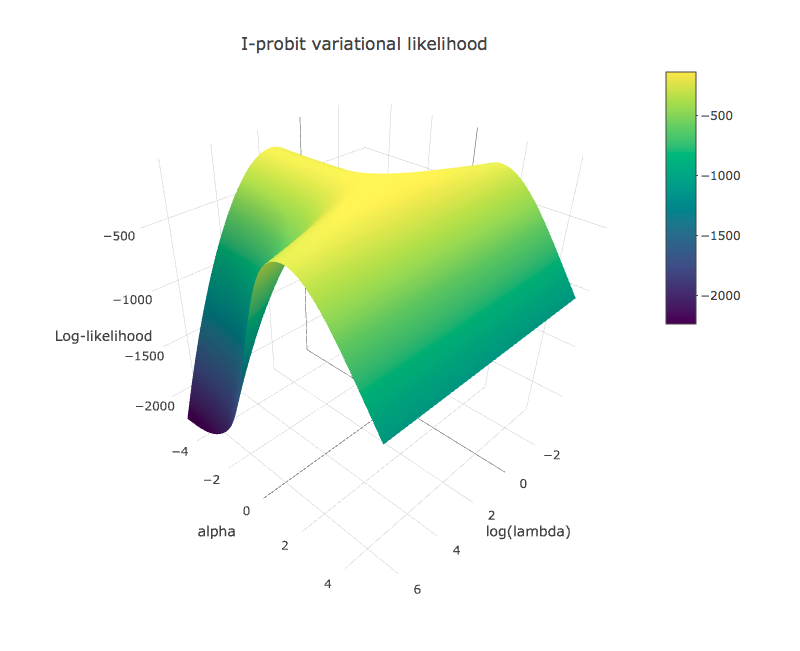
\includegraphics[width=0.49\textwidth]{figure/05-lik_vi}
  \vspace{1em}
  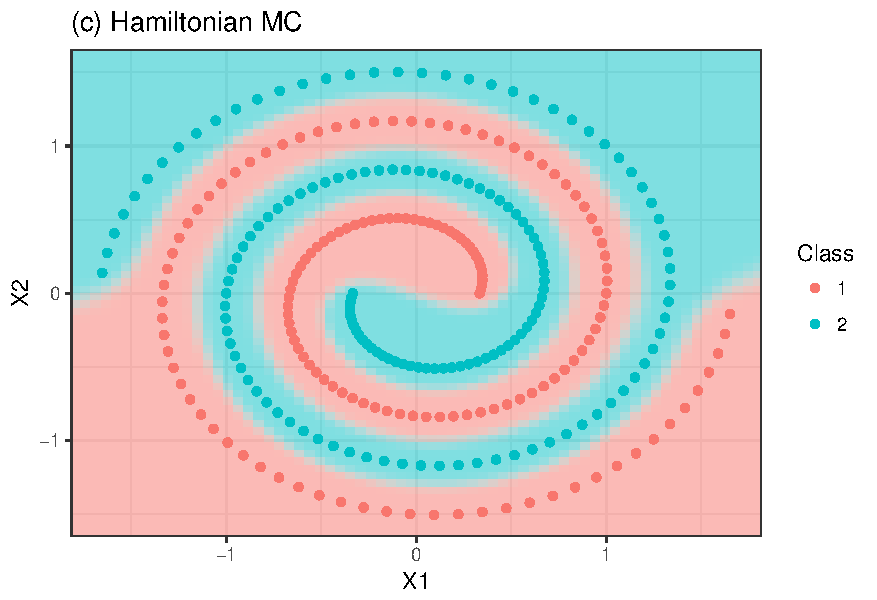
\includegraphics[width=0.49\textwidth]{figure/05-fit_hmc}
  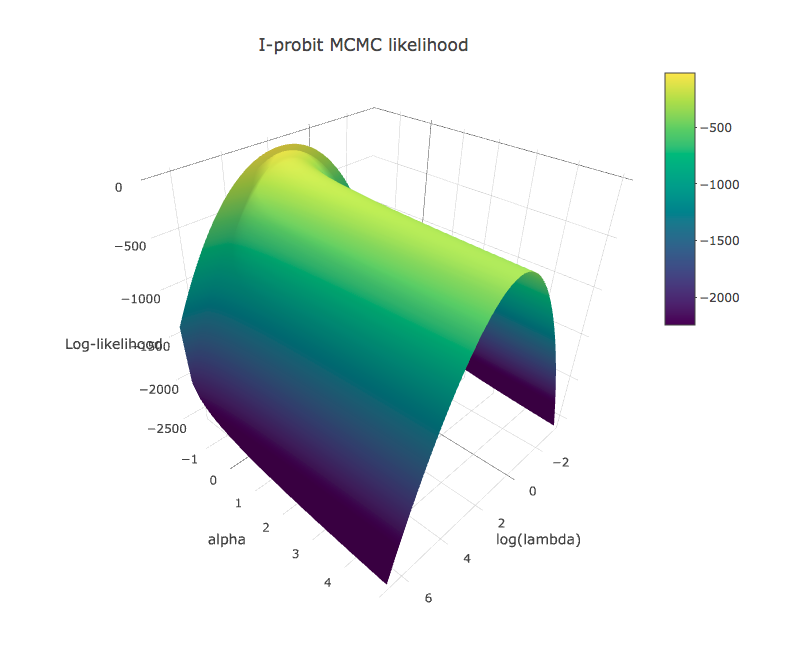
\includegraphics[width=0.49\textwidth]{figure/05-lik_hmc}
  \caption{Plots showing predicted probabilities (shaded region) for belonging to class 1 or 2 indicated by colour and intensity, and likelihood surface plots for (a) Laplace's method, (b) variational inference, and (c) Hamiltonian MC.}
  \label{fig:exampleiprobitfit}
\end{figure}
